\section{Overview}
For the last decade, the common paradigm in the use of deep learning has been to improve model performance by improving architecture and scale. These models, feature larger and larger layers that are highly interconnected, otherwise referred to as dense. While this approach has continuously led to improvements in model performance it is not without drawbacks. In 2011 a state-of-the-art computer vision model could run using a laptop. Now running a state-of-the-art language mode requires a cluster of specialized GPUs which can cost upwards of \$100,000 dollars and draw kilo-watts of power. \\
Inspired by the sparsity of the connections of neurons in the brain, unstructured sparsity seeks to improve the model efficiency by turning densely connected models into sparse models which as a result are far more efficient. While a large portion of existing research has focused on theory and high-level implementations our work is focused on using the same sparsity to realize true measurable inference speedups. 
\section{The Optimal BERT Surgeon: Scalable and Accurate Second-Order Pruning for Large Language Models}
\subsection{Overview}
Pre-trained Transformer-based language models have become a key building block for natural language processing (NLP) tasks. While these models are extremely accurate, they can be too large and computationally intensive to run on standard deployments, such as commodity CPUs. A variety of compression methods, including Knowledge Distillation (KD), quantization, structured and unstructured pruning have all proven to be effective for decreasing model size and increasing inference speed. Yet, research on these methods is still at an early stage, and little is known concerning the potential and limitations of applying these methods in conjunction.  
In this section, we introduce a general framework for \emph{compounding} compression approaches for Transformer-based models, which allows us to combine structured and unstructured pruning together with quantization, in order to obtain highly-compressed, but accurate models.   
We apply our approach to transfer tasks, generating compressed models that can be up to $\sim$ 9x smaller; 
paired with a sparsity-aware CPU inference engine, we obtain inference throughput improvements of over 7x on CPUs, all with negligible loss in accuracy 
\section{Sparse*BERT: Sparse Models Generalize To New tasks and Domains}
\subsection{Overview}
Large Language Models have become the core architecture upon which most modern natural language processing (NLP) systems build. These models can consistently deliver impressive accuracy and robustness across tasks and domains, but their high computational overhead can make inference difficult and expensive. To make the usage of these models less costly recent work has explored leveraging \textit{unstructured pruning} to improve inference speed and decrease size. This paper studies how models pruned using Gradual Unstructured Magnitude Pruning can transfer between domains and tasks. Our experimentation shows that models that are pruned during pretraining using general domain masked language models can transfer to novel domains and tasks without extensive hyperparameter explorations. We demonstrate that our general sparse model \textit{Sparse*BERT} can specialize simply by pretraining the compressed architecture on unstructured biomedical text to become SparseBioBERT. SpaseBioBERT is able to match and exceed the performance of BioBERT with 10\% of the parameters.
\subsection{Introduction}
Foundational Models \cite{Bommasani2021OnTO} based on the Transformer architecture \cite{Vaswani2017AttentionIA} have quickly become the most common building block in the modern language understanding stack, providing robust language representations which can be leveraged by to provide impressive accuracy on tasks like question answering, text classification, and token classification. These Large Language Models (LLMs) have shown to be robust to shifts in domain and domain specific models like BioBERT \cite{Lee2020BioBERTAP}, LEGALBERT \cite{Chalkidis2020LEGALBERTTM}, and SCiBERT \cite{beltagy2019SciBERTAP} have become a popular strategy for improving performance further. While accurate and robust, LLMs are not without drawbacks. They commonly have hundreds of millions or billions of parameters which generally require large specialized computer clusters to run inference at scale. Several approaches have been successfully used to improve performance of these LLMs, such as approximating attention \cite{Peng2021RandomFA}, removing portions of the models \cite{Sridhar2020UndividedAA} and reducing the precision of activation and weight values.\\
\begin{figure}[!
t]
    \centering
    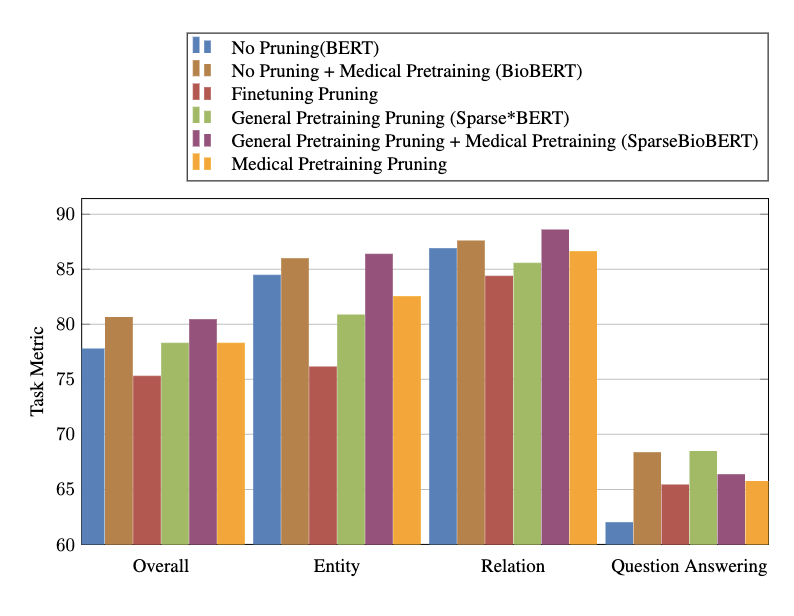
\includegraphics[scale=0.8
    ]{media-sparse/sparseBIO-figure1.png}
    \vspace{-1.2em}
\caption{Impact of stage and domain of pruning when evaluating BERT base uncased on medical NLP Entity Extraction, Relation Extraction, and Question Answering. For pruned and unpruned models medical pretraining can improve performance and the performance of the pruned model and the performance of BioBERT and SparseBioBERT is equivalent.}
\label{fig:sparse_transfer_categorical}
\end{figure}
Recent work \cite{Zafrir2021PruneOF} \cite{Kurti2022TheOB} has shown that the application of unstructured and semi-structured (block) pruning mechanisms on LLMs can significantly compress models with little to no loss in accuracy. While these approaches are successful and applicable during model general pretraining and task-specific fine-tuning, prior work has not studied how pruned models transfer to novel domains nor the impact of pretraining stage pruning on transfer accuracy. Given that most applications would require transfer of the general LLMs to a specific application domain, it is important to study the generality and robustness of the pruned LLMs when they are applied to multiple tasks in an application domain.  \\
In our work, we focus on studying how generalizable pruned LLMs are by evaluating how well they are able to transfer to previously unstudied tasks in a a new domain.
Specifically, we study these questions by focusing on transferring pruned and unpruned LLMs to the biomedical domain and evaluating the accuracy of said models on downstream tasks like Entity Extraction(EE) and Relation Extraction(RE), and Question Answering(QA). Our experiments demonstrate that pruned LLMs generalize well and are robust to domain transfer and variation in target task, dataset size, and dataset difficulty. In summary, our contributions are as follows:
\begin{itemize} 
\item We demonstrate that LLMs pruned on the general domain language can transfer to novel domains without extensive hyperparameter tuning and can produce equivalent or better accuracy when compared to dense LLMs.
\item We introduce a sparse model, Sparse*BERT, and its domain adaptation adapted for the Medical/Bio NLP domain called SparseBioBERT. This model matches the accuracy of the BioBERT with $10\%$ of the active parameters.
\end{itemize}
\subsection{General Sparse Models Can Adapt to Novel Domains}
While existing pruning research has found it possible to prune models heavily without loss in accuracy, most approaches have focused on the compression of individual tasks or textual domains. These specialized models match or exceed the accuracy of the dense model but commonly require vast amounts of hyperparameter turning and task-specific optimization to achieve this result. Compressed models like DistillBERT \cite{Sanh2019DistilBERTAD}, and TinyBERT \cite{Jiao2020TinyBERTDB} are some of the most popular LLMs because they provide compression without any additional know-how or optimization. For pruned models to become a common architecture for NLP tasks these models must be as robust and easy to use as their uncompressed counterparts. \\
In this paper, we explore this potential and propose 
Sparse*BERT, a novel pruned LLM that can adapt effectively to novel domains without extensive fine-tuning or task-specific pruning.\\
We can formulate the Sparse*BERT model as $\theta^*$, which can approximate the accuracy of the dense model $\theta$ and does not suffer model collapse when transferred to novel domains. The architecture of Sparse*BERT matches BERT, but a portion of its weights are pruned and masked to avoid future updates. To ensure that our sparse model can approximate the accuracy of the dense model, we leverage Knowledge Distillation by comparing the relative entropy using the Kullback–Leibler divergence between the outputs of the dense and sparse networks.   \\
Following the success of Zafrir et al. \cite{Zafrir2021PruneOF} we leverage Gradual Magnitude Pruning (GMP) to introduce sparsity into language models. To ensure that we can maximize the inference speedups, we prune each set of components in the network independently. The structure in the model graph groups these components, so the individual feed-forward layers, the queries, or keys, but not individual self-attention heads. 
\subsection{Methodology}
To assess how well-pruned models can transfer to novel domains and determine the optimal stage of pruning (pretraining, domain transfer, or fine-tuning), we evaluate the accuracy on 10 Biomedical biomedical datasets. Our experiments fix the training parameters for all the transfer tasks and vary the stage used for pruning (no pruning, pretraining, domain transfer, fine-tuning) and domain-specific pretraining.
\subsubsection{Datasets}
In all of our experiments we focus on English only biomedical datasets/corpora. Each dataset that we use is unmodified from its described use in the literature and its associated and prescribed metrics are used.\\
\textbf{Pretraining Datasets.} To understand how the stage of pruning impacts model accuracy, we train models both pruned and dense models on the Medline/PubMed corpus and the combination of English Wikipedia \cite{wikidump} and The Book Corpus \cite{Zhu_2015_ICCV} datasets. \\
The combination of Wikipedia and Book Corpus dataset creates a common domain language dataset featuring ~3.3 billion words which have become the backbone for experimentation for general domain masked language modeling. \\
The MEDLINE/PubMed Corpus is a publicly available\footnote{https://www.nlm.nih.gov/databases/download/pubmed\_medline.html} text corpus made up of journal abstracts and documents of biomedical literature from around the world. The corpus is updated daily by the United States National Institute of Health and it has been the primary resourced used to train BioMedical LLMs like BioBERT \cite{Lee2020BioBERTAP} and PubmedBERT \cite{Gu2022DomainSpecificLM}. For our experiments, we extracted our corpus on January 2022, and filter and prepare the dataset for masked language modeling using the BioElectras \cite{Kanakarajan2021BioELECTRAPretrainedBT} scripts\footnote{https://github.com/kamalkraj/BioNLP-Corpus}. This formatted PubMed corpus has 34,246,348 abstracts and 4.5 billion words \cite{Kanakarajan2021BioELECTRAPretrainedBT}. \\
\begin{table}[!ht]
    \centering
    \scalebox{0.7}{ 
    \begin{tabular}{c|c|c|ccc|c}
    \toprule 
    Dataset & Domain & Task Type & Training Size & Testing Size & Validation Size & Evaluation Metric \\
    \midrule
    BC5-Chem & Medical & Entity Recognition & 5203 & 5347 & 5385 & F1 \\ 
    BC5-disease & Medical & Entity Recognition. & 4182 & 4244	 & 4424	 & F1 \\
    NCBI-disease & Medical & Entity Recognition & 5134 & 787 &	960 & F1 \\
    BC2GM	& Medical & Entity Recognition & 15197 &	3061 &	6325 & F1 \\ 
    JNLPBA	& Medical & Entity Recognition & 46750 &	4551 &	8662 & F1 \\	
    ChemProt & Medical &	Relation	& 18035 & 	11268	& 15745	& F1 \\
    DDI	& Medical & Relation	& 25296	&2496 &	5716 & F1 \\
    GAD & Medical&	Relation	&4261	& 535 &	534	 & F1 \\
    PubMedQA & Medical &	Question Answering &	450 &	50 &	500 &	Accuracy \\
    BioASQ	& Medical & Question Answering &	670	 & 75	& 140 &	Accuracy \\
    SQUAD & General & Question Answering & 87599& 10570 & N/A & F1  \\ 
    \bottomrule
    \end{tabular}
    }
    \caption{In order to understand how generalizable sparse models are we evaluate on a wide set of tasks that vary in difficult, size, and desired output}
    \label{tab:dataset_descriptions}
    \vspace{-1.2em}
\end{table}
\textbf{Finetuning Datasets.} We finetune pretrained models on 10 established BioMedical NLP datasets, encompassing 3 separate task types: Entity Recogniton (ER), Releation Extraction (RE), and Question answering (QA). For ER we use the BioCreative II Gene Mention Recognition (BC2GM), \cite{Smith2008OverviewOB}, BC5CDR Drug/Chemical (BC5-Chem), BC5CDR Disease (BC5-Disease) \cite{Li2016BioCreativeVC}, JNLPBA \cite{Collier2004IntroductionTT}, and NCBI Disease \cite{Dogan2014NCBIDC} datasets. For RE we use ChemProt \cite{Taboureau2011ChemProtAD}, Drug-Disease Interaction (DDI) \cite{HerreroZazo2013TheDC}, and Gene-Disease Associations (GAD) \cite{Becker2004TheGA} datasets. For QA we leverage BioASQ task 7B \cite{Baker2016AutomaticSC} and  PubMedQA \cite{Jin2019PubMedQAAD}. In addition, we perform an analysis of the impact of the size of the finetuning dataset on the optimal stage for pruning using the non biomedical QA SQUAD \cite{Rajpurkar2016SQuAD1Q} dataset. Details on dataset size, evaluation metric and domain can be found in Table \ref{tab:dataset_descriptions}.
\subsubsection{Experimental Setup}
Our experiments focus on the popular BERT-base-uncased language model \cite{Devlin2019BERTPO}, which is an LLM composed of 12 transformer encoder layers and has 110M parameters. Following previous work, we do not prune the embedding layers of the network or any task-specific heads and focus on the $\sim\!85$ million parameters found in the encoder layers. To ensure that our experiments are reproducible \footnote{we will be releasing our code and models to allow reproduceability and extensibility} we use the popular open-source libraries SparseML \footnote{https://github.com/neuralmagic/sparseml} and Transformers \footnote{https://github.com/huggingface/transformers}. \\
\textbf{Model Pretraining}
Pretraining refers to the stage in which the model is trained on an unsupervised NLP dataset using a masked language modeling (MLM) approach \cite{Devlin2019BERTPO}. Pretrained models are fine-tuned on labeled task-specific datasets to optimize for task-specific accuracy.
For our experiments, we use existing dense pretrained models for BERT-base-uncased \cite{Devlin2019BERTPO} and PubmedBERT \cite{Gu2022DomainSpecificLM} and prune them using gradual magnitude pruning based on the corresponding dataset and MLM approach. Details about pruning regimes and hyperparameters can be found in the appendix.
During model pretraining, we train for three epochs on 4 A100 GPUS using a batch size of 256, the sequence length of 512, and, following early experiments and findings from Kurtic et al.\ and Zafir et al., we cycle the learning rate during pretraining and found cycling twice per epoch from 5e-4 to 0 to be most effective. First, we take the existing dense models and run this training setup for 3 epoch to ensure there is model convergence, then taking these converged models, we retrain and apply gradual magnitude pruning over the first two epochs. During pruning, we start from an initial sparsity of $30\%$ and gradually pruning to a final sparsity of 90\% pruning 100 times an epoch. After model pruning, we continue to train for one additional epoch to ensure that the sparse model is converged.  \\
Based on early experiments, we find knowledge distillation beneficial. For all of our experiments in pretraining, we leverage well-trained dense teachers using a hardness of  0.5 and a temperature of 2. When pruning weights, their values are fixed to 0 and are masked to avoid future updates. Effectively this means that our experiments evaluate the discovery of the most optimal sub-architecture. \\
\textbf{Model Finetuning}
Finetuning refers to the stage in which the model is trained on a supervised NLP dataset using a task specific training regime. In this stage one or many classification heads are connected the the model and a these classification heads and the pretrained model are trained for optimal performance on an individual task.
To isolate the effects of task-specific hyperparameter tuning and pruning stages, we fix the training procedure across fine-tuning tasks. Specifically, we train each model for ten epochs on a V100 GPU using a batch size of 16, a learning rate that linearly decays from 5e-5, and replicates using five random seeds for larger tasks and ten random seeds for smaller tasks. \\
We use the same setup both for fine-tuning already pruned models and when applying gradual magnitude pruning during fine-tuning (pruning on the fine-tuning stage). For pruned models, we preserve the sparsity patterns. When pruning models during fine-tuning, we fine-tune the dense model for two epochs, prune over the preceding six epochs, and stabilize the pruned network for two epochs. In our early experiments and matching prior findings \cite{Zafrir2021PruneOF}, we find that when pruning models on transfer tasks, accuracy is best when the learning rate cycles. Cycling only occurs when pruning during fine-tuning, and the learning rate cycles at epochs 2 (start of pruning) and 8 (end of pruning). Unlike previous work, we do not find a significant effect in accuracy improvement by leveraging knowledge distillation on the fine-tuning task. As a result, we do not use knowledge distillation during fine-tuning.
\subsection{Experimental Discussion}
\begin{table}[h!]
    \centering
    \scalebox{0.8}{ 
    \begin{tabular}{c|c|ccc|c}
    \toprule 
    Model & Pruning Stage &  EE & RE & QA & Overall \\
    \midrule
    BERT-Base-Uncased & \makecell{None \\ Fine tuning \\ Pretraining} & \makecell{\textbf{84.44}  \\ 76.12 \\ 80.84}  & \makecell{\textbf{86.86} \\ 85.36 \\ 85.54} & \makecell{61.97 \\ 65.39 \\ \textbf{68.44}} & \makecell{77.76 \\ 75.28 \\ \textbf{78.27}}\\
    \midrule
    BioBERT-Base-Uncased &  \makecell{None \\ Fine tuning \\ Pretraining (Medical)\\ Pretraining (General)} & \makecell{85.96 \\ 63.53 \\ 82.50 \\ \textbf{86.36}} & \makecell{87.56 \\ 75.14 \\ 86.60 \\ \textbf{88.57}}  & \makecell{\textbf{68.33}\\  54.00 \\ 65.71 \\ 66.33} & \makecell{\textbf{80.62} \\ 66.34 \\ 78.27 \\ 80.42}  \\
    \bottomrule
    \end{tabular}
    }
    \caption{Overall results on the impact of task and dataset of model pruning. Models trained for the general domain and pruned on the general domain can transfer at equal or better accuracy. Question Answering is the notable outlier as its small dataset size benefits from the sparse models as their pruned architecture prevents overfitting on small datasets.}
    \label{tab:full_datasets}
    \vspace{-1.2em}
\end{table}
\begin{table}[htb!]
    \centering
    \scalebox{0.5}{ 
        \begin{tabular}{cc|ccccc|ccc|cc}
    \toprule 
    Model & Pruning Stage & BC5-Disease & BC5-chem & NCBI-disease & BC2GM & JNLPBA & ChemProt & DDI & GAD & \makecell{PubMedQA \\ Accuracy} & \makecell{BioASQ \\ Accuracy} \\
    \midrule
    Training dataset size & N/A& 4182 & 5203 & 5134 & 15197 & 46750 & 18035 & 25296 & 4261 &  450 & 670 \\
    \midrule
    BERT-Base-Uncased & \makecell{None \\ Fine tuning \\ Pretraining}  & \makecell{80.60 \\ 69.87 \\ 75.35} & \makecell{91.23 \\ 81.72 \\ 87.83} & \makecell{\textbf{85.66}\\ 75.57 \\ 81.75 } & 
    \makecell{81.97 \\ 74.27 \\ 77.12} & \makecell{81.56 \\ 79.57 \\ 81.24}  &  \makecell{88.19 \\ 85.41 \\ 86.13} & \makecell{94.35 \\ 92.72\\ 92.73} & \makecell{78.05 \\ 74.88 \\ 77.77}  & \makecell{47.46 \\52.67 \\ 50.00} & \makecell{76.65 \\ 78.11 \\ 82.89} \\
    \midrule
    BioBERT-Base-Uncased &  \makecell{None \\ Fine tuning \\ Pretraining(General) \\ Pretraining(Medical)}  &\makecell{83.195 \\ 66.34 \\\textbf{83.32} \\ 80.56 } &  \makecell{93.63 \\ 66.60 \\ \textbf{93.81} \\92.17 } & \makecell{83.46 \\ 52.69 \\ 84.15 \\ 78.84}&  \makecell{86.05 \\ 59.71 \\\textbf{87.04} \\ 81.11} &  \makecell{\textbf{84.10} \\62.15 \\ 81.84 \\ 81.81 } &   \makecell{90.66 \\ 80.28 \\ \textbf{90.71} \\ 88.02} &  \makecell{95.01 \\ 87.60  \\ \textbf{95.02} \\ 93.99} &  \makecell{77.02 \\ 57.55 \\ \textbf{79.90} \\ 77.77} &   \makecell{\textbf{54.00}\\ \textbf{54.00} \\ 51.50 \\ 49.14} &  \makecell{\textbf{82.67}\\ \textbf{82.67} \\ 81.17 \\ 82.28} \\
    \bottomrule
    \end{tabular}
    }
    \caption{Performance on Complete set of tasks. Except for question answering tasks and NCBI-Disease, the SparseBioBERT outperforms all other models, including BioBERT, indicating that sparse architectures can be transferred to novel domains and use cases without additional optimization. }
    \label{tab:full}
    \vspace{-1.2em}
\end{table}
When we evaluate results on an average of task specific scores as shown in Table \ref{tab:full_datasets} we can see that the SparseBioBERT model performs on par with the its unpruned counter-part and outperforms it on relation extraction and entity extraction. Results on individual tasks can be found in the appendix in Table \ref{tab:full} and further consistently show how SparseBioBERT approximated BioBERT. When pruned models do not transfer to the biomedical domain they can perform much worse than the unpruned models as shown by the sizable gap in between the pruned and dense BERT-base-uncased models. This result, coupled with the performance of SparseBioBERT makes us believe that pruned models are able to adapt to new domains like unpruned models but require additional domain specific pretraining to ensure performance. \\
We believe that these results provide evidence that models pruned during general domain language modeling can remove large portions of the model without affecting the ability to transfer to novel domains or tasks. Unlike pruning on specific domains and tasks, general domain pruning can preserve accuracy invariant to task and domain. \\
Unexpectedly, when evaluating biomedical QA, we improve accuracy with pruned models when pruned but only on a regular BERT model pruned downstream or the general domain Sparse*BERT. \\ We attribute this to the regularizing effect that pruning can have, and it likely helps in overfitting on small datasets, PubMedQA and BioASQ. Tasks. Finding that models pruned during outperform all others, we believe the regularization provided by pruning can prevent the overfitting on these small datasets.  \\
Our results also indicate that it is optimal to prune on general domain language modeling and transfer to novel tasks and domains for optimal performance. Regardless of their domain expertise, BERT and BioBERT both see huge losses in accuracy when pruned on the downstream tasks, and these same losses are not found in the model pruned during pretraining. Surprisingly, the model pruned on general domain language modeling outperforms when pruned on the biomedical domain-specific language modeling. this gap is nearly 4 points on entity extraction and 2 points overall, almost more significant than the gap between the BERT and BioBERT. \\
When we evaluate the impact of pruning on individual tasks pruning in fine-tuning stage) as shown in Table \ref{tab:full}, we can see that pruning is quite sensitive to the dataset task. Looking at the large datasets like JNLPBA in Table \ref{tab:full}, there is nearly no distinction in pruning during pretraining or fine-tuning. On the other hand, small datasets like NCBI and GAD see a large accuracy loss from models pruned during fine-tuning. In our appendix we describe further experiments to evaluate the impact of variations in dataset size on SQUAD \cite{Rajpurkar2016SQuAD1Q} finding that models pruned during pretraining behave like unpruned models while slightly less sample efficient.
\subsection{Impact of Training Data Size}
Noting that there is a significant variation in dataset size in the biomedical NLP tasks, we leveraged a dataset well studied in pruning, SQUAD, and performed variations to the training data size. Starting with the initial training dataset size, 88,000 items, we decreased the size to $75\%$,$50\%$,$25\%$,$10\%$,$5\%$,$2\%$,$1\%$ and evaluated the impact to performance. We compared the dense BERT, Sparse*BERT, and pruning BERT during fine-tuning. The sparse models each have $90\%$ unstructured sparsity on the encoder portion of the LLM. \\ 
Each experiment was performed with five random seeds, using a batch size of 12, and trained for 30 epochs with a learning rate decaying linearly from 5e-5 to 0. Each model's training uses knowledge distillation from a dense teacher with the hardness set to 0.8 and the temperature to 2.0. For the model pruned during fine-tuning, we cycle the learning rate at the beginning of pruning(2nd epoch) and the end of pruning(20th epoch). We evaluate model performance on the F1 score on the unaltered dev portion of the SQUAD dataset to avoid losses in evaluation sensitivity.\\
As shown in Figure \ref{fig:squad_data_size} and Table \ref{tab:squad_dataset} results in the appendix, models which are pruned during finetuning are not robust to variations in data size. Model performance decays slowly from 85 to 80 until the training data is decreased by $75\%$, but when it becomes smaller than that, it quickly becomes nearly unusable. The same cannot be said about the dense or the Sparse*BERT model as they see virtually identical losses in quality from 
\begin{figure}
   \centering
    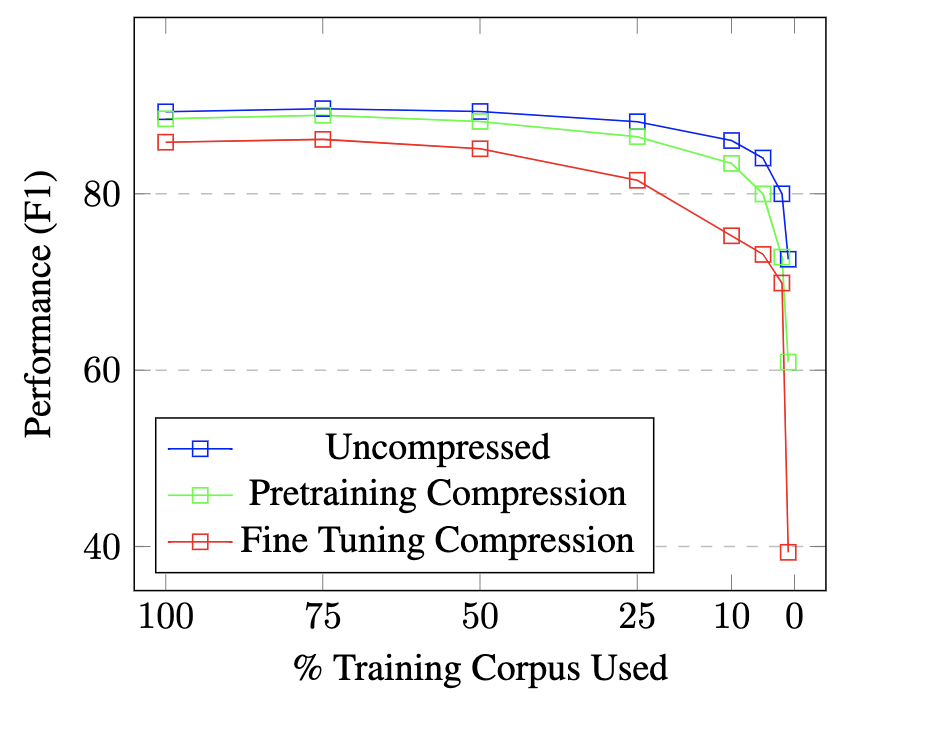
\includegraphics[scale=0.5
    ]{media-sparse/sparseBIO-figure2.png}
    \vspace{-1.2em}

\caption{Impact of varying the training data size with pruned and dense models showcases how pretraining pruning has a similar accuracy to the dense models.}
\label{fig:squad_data_size}
\end{figure}
\begin{table}[htb!]
    \centering
    \scalebox{0.9}{ 
    \begin{tabular}{|c|ccc|}
    \toprule 
     Training Data Portion& BERT-BASE-Uncased  &  Sparse*BERT & Finetune Pruning \\
    \midrule
    100 & 89.30 & 88.50 & 85.852 \\ 
    75 & 89.65 & 88.91 & 86.17 \\
    50 & 89.33 & 88.21 &  85.11 \\
    25 & 88.17 & 86.48 & 81.5 \\
    10 & 86.04 & 83.45 & 75.24 \\
    5 & 84.06 & 79.99 & 73.13 \\
    2 & 80.00 & 72.83 & 69.88 \\
    1 & 72.58 & 60.91 & 39.35 \\
    \bottomrule
    \end{tabular}
    }
    \caption{Model accuracy as measured by F1 on dev portion of SQUAD compared to model type and the impact of training data size. Sparse models are not as sample efficient as their dense counterparts, but Sparse*BERT performance matches the dense model much more than the model pruned downstream.}
    \label{tab:squad_dataset}
    \vspace{-1.2em}
\end{table}
\subsection{Limitations and broader impact}
Our approach is limited in the computational time required to generate a general sparse LLM and the diversity of type of LLMs that we explore. \\
In terms of computational expense, training a sparse model requires non negligible additional compute which is tractable for models with a hundred million parameters and a few billion tokens not for billion parameter models commonly discussed. \\
In terms of our current explorations our current explorations have been limited to monolingual LLMs trained on English. It is unclear how well sparse architectures will perform in a multi lingual setting and we expect degradation in language quality to be anything but equal across all languages. \\
\subsection{Conclusion}
In this work, we have introduced Sparse*BERT, a pruned LLM which builds on successful pruning algorithms research and demonstrates its ability to transfer to novel domains and tasks without additional hyperparameter search. Our experiment demonstrates how well Sparse*BERT can transfer to the biomedical domain to become SparseBioBERT. SparseBioBert can match the performance of BioBERT with $\frac{1}{10}$ of the parameters and no additional task-specific optimization. 
\section{Current Work}
Currently, we have been working on expanding our approaches in generating sparse language models for efficiency with our proposed work: OBERTA. OBERTA builds on our prior work on leveraging unstructured sparsity for efficiency inference but is able to provide large gains in accuracy because of our use of more optimized dense language models, improved distillation and training regimes, and optimized Quantization workflows. As shown in table \ref{tab:OBERTA-squad} our OBERTA 90\% model exceeds the performance of existing sparse 24 transformers layer sparse models despite being half the size. Our OBERTA 95\% model is able to exceed the performance of existing sparse 12-layer models with 5\% higher sparsity. We will expand this work to include structurally pruned models, improved quantization, and benchmarking on a wide variety of datasets such as SQUAD v1.1 \cite{Rajpurkar2016SQuAD10} and SQUAD v2.0 \cite{Rajpurkar2018KnowWY} for question answering, QQP \footnote{https://quoradata.quora.com/First-Quora-Dataset-Release-Question-Pairs} and MNLI \cite{Williams2018ABC} for  text classification, SST-2 \cite{Socher2013RecursiveDM} for sentiment analysis, IMDB for document Classification \cite{Maas2011LearningWV}, and CONLL2003 \cite{Sang2003IntroductionTT} for token classification.
\begin{table}[!ht]
    \centering
    \begin{tabular}{|l|l|l|l|}
    \hline
        Model & Sparsity & Transformer Layers & SQUAD F1  \\ \hline
        BERT base & 0 & 12 & 88.54  \\ \hline
        BERT Large & 0 & 24 & 90.93   \\ \hline
        Prune OFA Base & 90 & 12 & 87.25  \\ \hline
        Prune OFA Large & 90 & 24 & 90.02\\ \hline
        OBERT & 90 & 12 & 88.31 \\ \hline
        OBERT & 90 & 24 & 89.96  \\ \hline
        SparseBERT & 80 & 12 & 82.5  \\ \hline
        OBERTA & 90 & 12 & 91.0 \\ \hline
        OBERTA & 95 & 12 & 89.14  \\ \hline
    \end{tabular}
    \caption{OBERTA 90\% outperforms models 2 times as large on the SQUAD v1.1 dataset.}
    \label{tab:OBERTA-squad}
\end{table}

\section{Experimentation Plan}
\scalebox{0.8}{
\begin{tabular}{r |@{\foo} l}
January 2023 & Write Up OBERTa \\
\end{tabular}
}
